We applied the UI2I transformation between a panchromatic modality, \ie, a wide-band thermal image, and a monochromatic modality, \ie, a narrow-band thermal image.
For ease of notation, we will use the subscript \emph{pan} to describe panchromatic data, and \emph{mono} for monochromatic.

\section{Physical estimator}

\subsection{Estimator modeling}
Based on the relationship between intensity levels of a thermal camera and the incident power, as described in equation \ref{eq:naiveAffineTrans}, we can seemingly infer an object's temperature directly from the thermal image intensity and vice versa.
However, when dealing with an uncooled (non-thermally stabilized) microbolometric camera, the coefficients in the equation are highly sensitive to the camera's intrinsic temperature. 
According to \cite{10.1117/1.OE.52.6.061304}, the dependency of those coefficients on the intrinsic temperature can be faithfully approximated by a third-order polynomial, concluding that a more accurate description of a pixel's intensity level is
\begin{equation} \label{IntensityVsTemperatures}
  I(T_\mathit{obj}, T_\mathit{int}) = p^{(0)}_c(T_\mathit{int}) + p^{(1)}_c(T_\mathit{int}) T^4_\mathit{obj}
\end{equation}
where $T_\mathit{obj}$ is the object's absolute temperature, $T_\mathit{int}$ is the camera's intrinsic temperature at the time of acquisition, and:
\begin{equation} \label{poly_formula}
  p^{(i)}_c(T_\mathit{int}) = \sum_{k=0}^3  c_{i,k} T_\mathit{int}^k
\end{equation}
where the superscript $^{(i)}$ indicates that the two polynomials in equation \ref{IntensityVsTemperatures} have different coefficients.
Plugging equation \ref{poly_formula} into \ref{IntensityVsTemperatures} and simplifying all of the terms gives:
\begin{equation} \label{eq:full_expr}
  \begin{split}
    I(T_\mathit{obj}, T_\mathit{int}) &= c_{0,0} + c_{0,1} \cdot T_\mathit{int} + c_{0,2} \cdot T^2_\mathit{int} \\
    & + c_{0,3} \cdot T^3_\mathit{int} + (c_{1,0} + c_{1,1} \cdot T_\mathit{int} \\
    & + c_{1,2} \cdot T^2_\mathit{int} + c_{1,3} \cdot T^3_\mathit{int}) \cdot T^4_\mathit{obj} \\
    &= <F, C>
  \end{split}
\end{equation}
where in the last transition, we factorize the relationship as an inner product by stacking all monomials in a single feature vector $F$ and all coefficients in a vector $C$.
Overall, the estimator in equation \ref{eq:full_expr} is made up of eight different monomials and parametrized by eight different corresponding coefficients.

\subsection{Estimator coefficient calibration}
\subsubsection{Calibration setup}
Equipped with the parametric term from equation \ref{eq:full_expr}, calibrating its coefficients will allow us to transform thermal image intensities to object temperatures and vice versa.
To accomplish this, we designed a calibration setup with the following components:
\begin{compactitem}
  \item an uncooled microbolometric camera; for our experiments, we used FLIR Tau2;
  \item an environmental chamber to control the camera's ambient temperature (which implicitly controls $T_\mathit{int}$), with an aperture drilled into one of its edges to allow for image acquisition from its interior;
  \item a blackbody target, essentially a flat-surface object whose temperature can be controlled with very fine precision, to control the temperature of the scene (\ie, $T_\mathit{obj}$);
  we used a scientific grade (CI SR-800N) extended-area black body.
\end{compactitem}
To collect measurements, the camera was mounted inside the environmental chamber facing the outside through the drilled aperture, and the blackbody target was placed in front of the camera outside the chamber, such that it covered the camera's entire field of view, as demonstrated in Figure \ref{calib_setup}.
\begin{figure}[H]
  \centering
  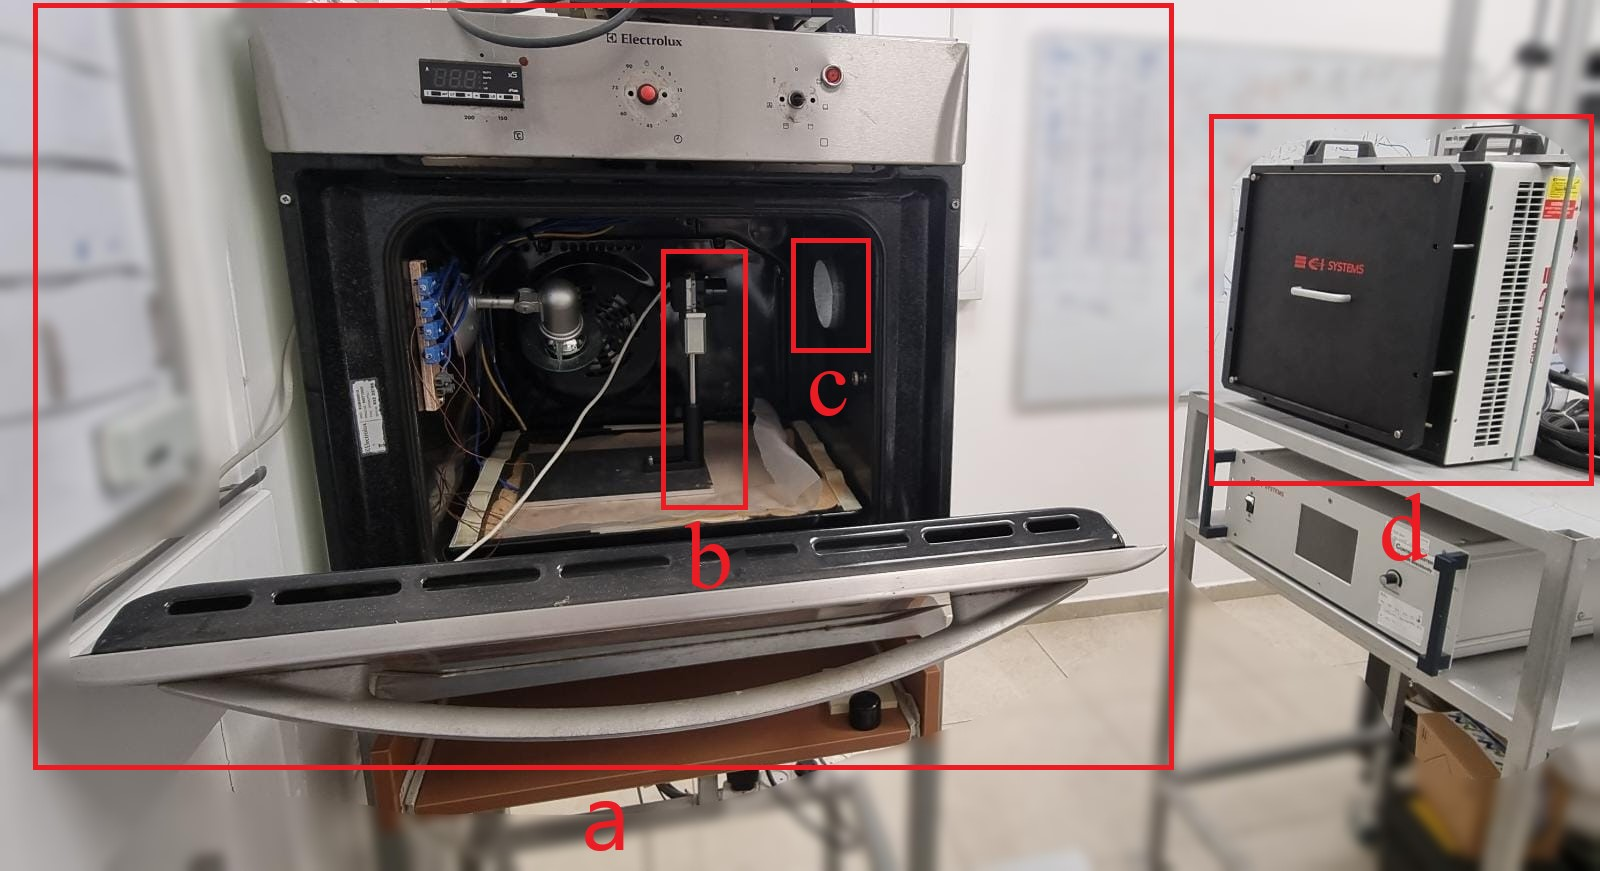
\includegraphics[width=\linewidth]{../figs/methods/calib_setup.jpg}
  \caption{The physical model-calibration setup. The black body target (d) is observed by the thermal camera (b) through a drilled aperture(c) at the edge of the environmental chamber (a). This setup enables controlling $T_\mathit{obj}$ and $T_\mathit{int}$ independently.}
  \label{calib_setup}
\end{figure}

\subsubsection{Coefficient extraction} \label{sec:coeff_extraction}
To efficiently estimate the coefficients, we organized the measured intensities and the coefficients in vectors $I$ and $C$ correspondingly, such that:
\begin{equation} \label{eq:matMult}
  \underbrace{
    \begin{pmatrix}
      1       & T_\mathit{int_{(0)}}  & \cdots & T_\mathit{obj_{(0)}}^4 T_\mathit{int_{(0)}}^3  \\
      1       & T_\mathit{int_{(1)}}  & \cdots & T_\mathit{obj_{(1)}}^4 T_\mathit{int_{(1)}}^3  \\
      \vdots  & \vdots                & \ddots & \vdots                                         \\
      1       & T_\mathit{int_{(N)}}  & \cdots & T_\mathit{obj_{(N)}}^4 T_\mathit{int_{(N)}}^3  \\  
    \end{pmatrix}  
  }_{M}
  \cdot
  \underbrace{
    \begin{pmatrix}
      c_{0,0} \\
      c_{0,1} \\
      \vdots  \\
      c_{1,3} \\    
    \end{pmatrix}  
  }_{c}
  = 
  \underbrace{
    \begin{pmatrix}
      I_{(0)} \\
      I_{(1)} \\
      \vdots  \\
      I_{(N)} \\    
    \end{pmatrix}  
  }_{I}
\end{equation} % TODO: need to make it fit in the paper (perhaps in appendix) 
where each row of the over determined matrix $M$ is the feature vector ($F$) of a single measurement, and $I$
holds the corresponding measured radiometric intensities.
Following the factorization from equation \ref{eq:full_expr}, the $n$th measured radiometric intensity equals the inner product between the $n$th measured feature vector and the vector of coefficients $C$:
\begin{equation}
  I[n] = <M[n, :], C> = <F[n], C>
\end{equation}
The matrix product factorization in equation \ref{eq:matMult} enables applying a linear regression to solve for the coefficients.
As the measurement noise appeared to be approximately white and Gaussian, the least-squares estimator (which is the maximum-likelihood estimator in the additive-white-Gaussian noise regime) was used to extract the coefficients:
\begin{equation} \label{eq:PseudoInverse}
  C = M^{\dagger} I
\end{equation}
where $M^{\dagger} = (M^TM)^{-1}M^T$ is the Moore-Penrose pseudoinverse of $M$.

In the calibration process described above, the intensity vector $I$ corresponds to a single pixel.
Because each element in the microbolometer might have a slightly different sensitivity, the coefficient extraction was performed independently for every pixel in the image.
The calibration results of an exemplary pixel can be visualized as a surface in the three-dimensional $T_\mathit{int}$-$T_\mathit{obj}$-intensity space, as shown in Figure \ref{physical_model_fit}.
\begin{figure}[H]
  \centering
  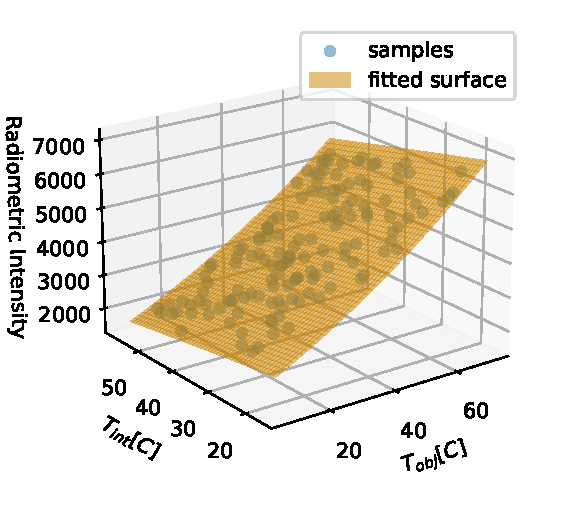
\includegraphics[width=0.7\linewidth]{../figs/methods/physical_model_tight.pdf}
  \caption{An example surface fit visualizing the calibrated polynomial coefficients of a single pixel.}
  \label{physical_model_fit}
\end{figure}

Based on equation \ref{IntensityVsTemperatures}, the calibrated coefficients can now be used to estimate the object's temperature using the panchromatic intensity and the intrinsic temperature at acquisition:
\begin{equation} \label{eq:backward_poly}
  \hat{T}_\mathit{obj} = \sqrt[4]{\frac{I_\mathit{pan} - p^{(0)}_{c_\mathit{pan}}(T_\mathit{pan})}{p^{(1)}_{c_\mathit{pan}}(T_\mathit{pan})}}
\end{equation}

\subsubsection{Measuring profile}
In order to achieve the best calibration results, 3 different measuring profiles were tested:
\begin{enumerate}
  \item $T_\mathit{int}$ ramp, $T_\mathit{obj}$ constant: 
  \begin{itemize}
    \item Environmental chamber temperature is monotonically increased from (cooled) room temperature until $T_\mathit{int}$ reaches 55C\textdegree.
    For Technical reasons, this is the only available profile for use by the environmental chamber.
    \item $T_\mathit{obj}$ is set to a constant operating point.
    \item The camera is set to acquire images in a constant frequency (\eg, every 2 seconds), to allow for some thermal variation to occur between subsequent acquisitions.
  \end{itemize}    
  As this method covers only one $T_\mathit{obj}$ per $T_\mathit{int}$ ramp, it requires repetition for several blackbody temperatures to properly cover the $T_\mathit{int}$-$T_\mathit{obj}$-intensity space.
  Since a temperature ramp takes a while to end (and cooldown takes even longer), this profile is very inefficient in time.
  Nevertheless, as the $T_\mathit{obj}$ remains constant throughout the process, the $T_\mathit{int}$ coverage per $T_\mathit{obj}$ is very dense, which is beneficial for the eventual coefficients regression (assuming sufficiently dense repetitions for different $T_\mathit{obj}$ operating points are used).

  \item $T_\mathit{int}$ ramp, $T_\mathit{obj}$ triangular wave:
  \begin{enumerate}
    \item Environmental chamber temperature follows the same profile as described in the first bullet (for \emph{$T_\mathit{int}$ ramp, $T_\mathit{obj}$ constant}).
    \item $T_\mathit{obj}$ is set to follow a triangular waveform, \ie, linearly increase between 10C\textdegree-70C\textdegree, and then decrease linearly in the opposite direction, then increase back again and so on and so forth, until $T_\mathit{int}$ reaches 55C\textdegree.
    \item The camera acquisition follows the same pattern as before.      
  \end{enumerate}
  This profile mitigates the need for many repetitions to some extent, as both $T_\mathit{obj}$ and $T_\mathit{int}$ change simultaneously within a single environmental chamber heating iteration.
  However, this comes in the expense of $T_\mathit{int}$ coverage per $T_\mathit{obj}$.

  \item $T_\mathit{int}$ ramp, $T_\mathit{obj}$ random:
  \begin{enumerate}
    \item Environmental chamber temperature follows the same profile as described in the first bullet (for \emph{$T_\mathit{int}$ ramp, $T_\mathit{obj}$ constant}).
    \item $T_\mathit{obj}$ is set to a random temperatures that are uniformely distributed between 10C\textdegree-70C\textdegree.
    \item The camera acquisition occurs after every stabilization of a randomly set $T_\mathit{obj}$.
  \end{enumerate}
  As was the case for \emph{$T_\mathit{int}$ ramp, $T_\mathit{obj}$ triangular wave}, this profile also mitigates the need for many repetitions.
  In contrast, and while for some $T_\mathit{obj}$ there is no $T_\mathit{int}$ coverage at all, the overall coverage of the $T_\mathit{int}$-$T_\mathit{obj}$-intensity space is much more uniform.
\end{enumerate}
A visualization of the measurements obtained by the 3 profiles in the 3-dimensional $T_\mathit{int}$-$T_\mathit{obj}$-intensity space appears in Figure \ref{fig:measrement_approaches}.
\begin{figure}[H]
  \centering
  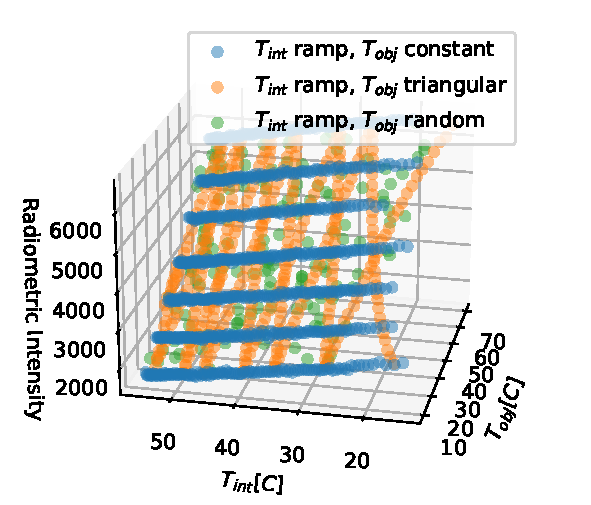
\includegraphics[width=0.7\linewidth]{../figs/methods/measurement_approaches.pdf}
  \caption{Surface fit visualizing the calibrated panchromatic polynomial coefficients for a randomly chosen pixel.}
  \label{fig:measrement_approaches}
\end{figure}

Evidently from figure \ref{fig:measrement_approaches}, the random profile yields the most uniform coverage of the $T_\mathit{int}$-$T_\mathit{obj}$-Intensity space, and thus is expected to yield the most accurate calibration results.
To validate this preliminary conclusion, the following steps were taken to compare between the different measurement profiles:  
\begin{itemize}
  \item The collected measurements of the different profiles were used to extract the coefficients per-pixel independently of eachother, resulting in three different sets of coefficients (one set per profile).
  \item An additional independent set of measurements were collected to evaluate and compare between the different profiles.
  \item The scene temperature of the images from the validation set was estimated using the extracted coefficients and equation \ref{eq:backward_poly}.
  \item The estimation error of all pixels from all images was used for the comparison.
\end{itemize} 
A histogram comparing the estimation error (\ie, the difference between the estimated $T_\mathit{obj}$ and the actual $T_\mathit{obj}$) obtained by each of the measurement profiles appears in Figure \ref{fig:profiles_error_comp}.
\begin{figure}[H]
  \centering
  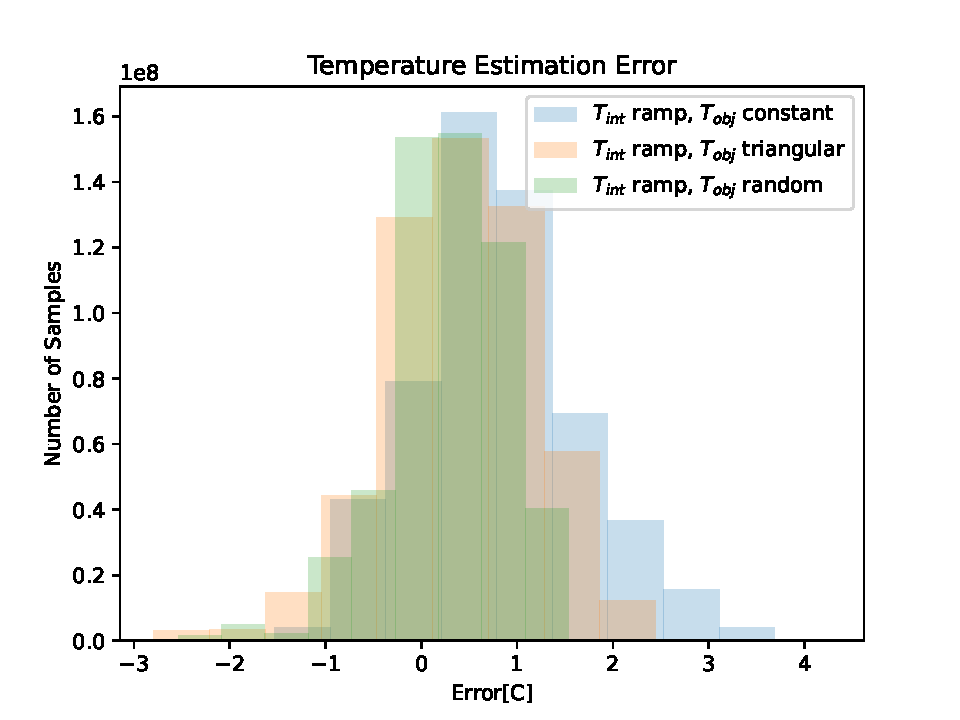
\includegraphics[width=\linewidth]{../figs/methods/profiles_error_comp.pdf}
  \caption{Histogram of the estimation error incurred by the different measurement profiles.}
  \label{fig:profiles_error_comp}
\end{figure}
Noticeably, the random $T_\mathit{obj}$ profile exhibits the tightest error distribution around zero, suggesting that it is the optimal measurement profile.
To make this argument more rigorous, significant error distribution statistics (mean, standard deviation (STD) and root-mean-squared error (RMSE)) were calculated and compared in Table \ref{tbl:meas_prof_err_stat}.
\begin{table}[H]
  \centering
  \begin{tabular}{| l || c c c |}
      \hline
      \multicolumn{1}{|c||}{Measurement Profile} & Mean & STD & RMSE\\
      \hline
      $T_\mathit{int}$ ramp, $T_\mathit{obj}$ constant    & 0.81 & 0.85 & 1.18\\ 
      \hline
      $T_\mathit{int}$ ramp, $T_\mathit{obj}$ triangular  & 0.41 & 0.78 & 0.88\\ 
      \hline
      $T_\mathit{int}$ ramp, $T_\mathit{obj}$ random      & 0.27 & 0.61 & 0.66\\ 
      \hline
  \end{tabular}
  \caption{Comparison of the estimation error statistics incurred by the different measurement profiles.}
  \label{tbl:meas_prof_err_stat}
\end{table}
In accordance with our qualitative impression, it appears that the error statistics also indicate that the random $T_\mathit{obj}$ profile is indeed the optimal one.
Therefore, we chose to use the random measurement profile as our standard for the rest of the activity.

\subsubsection{From panchromatic to monochromatic}
The main goal of this thesis is learning the I2I translation between panchromatic and monochromatic thermal images.
While multiple options are available for the monochromatic modality, we decided to focus on the a central wavelength of $9\mu m$ and full width at half maximum (FWHM) of $0.5 \mu m$.
From this point onward, we will refer to this part of the thermal bandwidth as the monochromatic modality.

As discussed and reflected by equation \ref{BolometerIncidentPower}, the relationship between the object's temperature and the image intensity depends on the camera's bandwidth.
Hence it is clear that the estimators coefficients extracted in the monochromatic setup (in which a narrow-band filter is applied over the lens) will be different from those extracted in the panchromatic setting, with a bandwidth of $7-14 \mu m$.
Therefore, the coefficient calibration was conducted twice, with and without applying an IR bandpass filter over the camera lens.

After estimating the object temperature using the extracted panchromatic coefficients and equation \ref{IntensityVsTemperatures} (which after simplifying reduces to \ref{eq:backward_poly}), we can invoke equation \ref{IntensityVsTemperatures} once again, this time using the extracted monochromatic coefficients, to estimate the monochromatic intensity:
\begin{equation} \label{eq:forward_poly}
  \hat{I}_\mathit{mono} = p^{(0)}_{c_\mathit{mono}}(T_\mathit{mono}) + p^{(1)}_{c_\mathit{mono}}(T_\mathit{mono}) \hat{T}_\mathit{obj}^4
\end{equation}
We treat the cascaded utilization of equations \ref{eq:backward_poly} and \ref{eq:forward_poly} as the physical estimator, and denote it by $G_{\mathit{phys}}$, that is:
\begin{equation}
  \hat{I}_\mathit{mono} = G_{\mathit{phys}}(I_\mathit{pan}, T_\mathit{pan}, T_\mathit{mono})
\end{equation}

% TODO: add Navot's image depicting the biased inaccuracy in temperature estimation
As it turns out, the calibrated physical estimator is not very accurate, and in particular suffers from a significant first-order error.
Those inaccuracies might have to do with issues related to the calibration setup, which would normally require an exhaustive investigation to find its root cause.
To circumvent this cumbersome effort, we apply a pixel-wise affine transformation to the estimator, \ie: 
\begin{equation}
  \tilde{G}_{\mathit{phys}} = A \circ G_{\mathit{phys}} + B
\end{equation}
where $A, B$ are matrices and $\circ$ is the Hadamard product operator.
By constructing the elements of the matrices $A, B$ as learnable parameters, backpropagation can be utilized to implicitly correct the physical estimator's prediction of the monochromatic output.

\section{Deep estimator}
Given the calibrated physical estimator, one might wonder why this is not enough to solve the UI2I task altogether. 
Unfortunately, as evident from equation \ref{stephan-boltzmann-practical}, the emissivity can utterly change the incident thermal radiation on the camera's sensor. 
Therefore, two objects sharing the exact same temperature might result in significantly different bolometric readouts, and thus different intensity levels \cite{holman1989heat}.
In addition, the application of an IR filter over the lens results in a scene-dependent spatial distortion known as the narcissus effect \cite{FundamentalsOfInfraredThermalImaging}.
This effect is easily observable in real monochromatic images, such as those in Figure \ref{fig:qual_comp} in the right-most column.
Hence, the physical estimator cannot accurately predict the intensity levels of a real-world scene, because it has no capacity to handle different object and scene conditions.
This is where the family of deep generative I2I translation models, which have significantly greater capacity than the polynomial physical estimator, is brought into play.
As baselines, we examined the architectures of CycleGAN \cite{CycleGAN2017} and CUT \cite{park2020cut}, which are considered to achieve SOTA results for the task of UI2I translation.
Both CycleGAN's and CUT's generators consist of a convolutional encoder-decoder scheme with a bottleneck of residual blocks \cite{He2016DeepRL} in between, as schematized in Figure \ref{fig:backbone_models}.

As previously stated in equation \ref{IntensityVsTemperatures}, the intensity levels of both our input and target modalities are affected by the camera's intrinsic temperature.
Fortunately, each image acquired by the FLIR Tau2 is saved along with the intrinsic thermal sensor readouts.
Specifically for our activity, we chose to use the focal plane array temperature as our intrinsic temperature ($T_\mathit{int}$).
Hence, it made sense to design an architecture that could accept this temperature as additional input.
More concretely, we provide the panchromatic (input) intrinsic temperature to the encoder, and the monochromatic (output) intrinsic temperature to the decoder\footnote{In CycleGAN, the generator translating back from the monochromatic to the panchromatic domain receives the inputs in the reverse order, \ie, monochromatic temperature to the encoder and panchromatic temperature to the decoder}.
In doing so, we attempt to disentangle the intrinsic-temperature-dependent transformations (handled by the encoder and decoder) and the more general inter-modal transformation (handled by the bottleneck).

Our use of the intrinsic temperatures as inputs can be thought of as an extension of the concept of conditional GAN (CGAN) \cite{mirza2014conditional}.
In our case, the output is conditioned on two continuous variables (panchromatic and monochromatic intrinsic temperatures) as opposed to the original paper where a single discrete conditional variable was used.
Since both the encoder and decoder are convolutional networks, the intrinsic temperatures (scalars) were reshaped as constant matrices before being concatenated to the corresponding tensors.

\section{Fusion of estimators} % TODO: see if there's room for flatter minima argument (also in the results)
Although somewhat mitigated by the learnable affine transformation, the calibrated physical estimator still suffers from inaccuracies.
Nevertheless, its prediction is much closer to the expected monochromatic output than a sheer random guess, which is the initial state of all ordinary GAN generators.
Hence, we can use the physical estimator to produce a prior approximation of the desired output, and let the deep estimator learn the residual \wrt the desired result.
This approach is expected to facilitate the deep estimator's pursuit of the optimal solution and thus improve its chances of converging to better and flatter local minima.
Therefore, our proposed method fuses the physical estimator (augmented with the affine transformation) with the deep estimator:
\begin{equation} \label{eq:genFuse}
  G_{\mathit{PETIT}}(x) = \tilde{G}_\mathit{phys}(x) + G_\mathit{deep}(x)
\end{equation}
where $G_\mathit{deep}$ is used to describe the generator of the deep estimator.
Schematics comparing the generator architecture of the deep baseline models (CycleGAN, CUT) and our model (PETIT) are shown in Figure \ref{fig:arch_comp}.

\begin{figure}[H]
  \centering
  \begin{subfigure}{\textwidth}
    \centering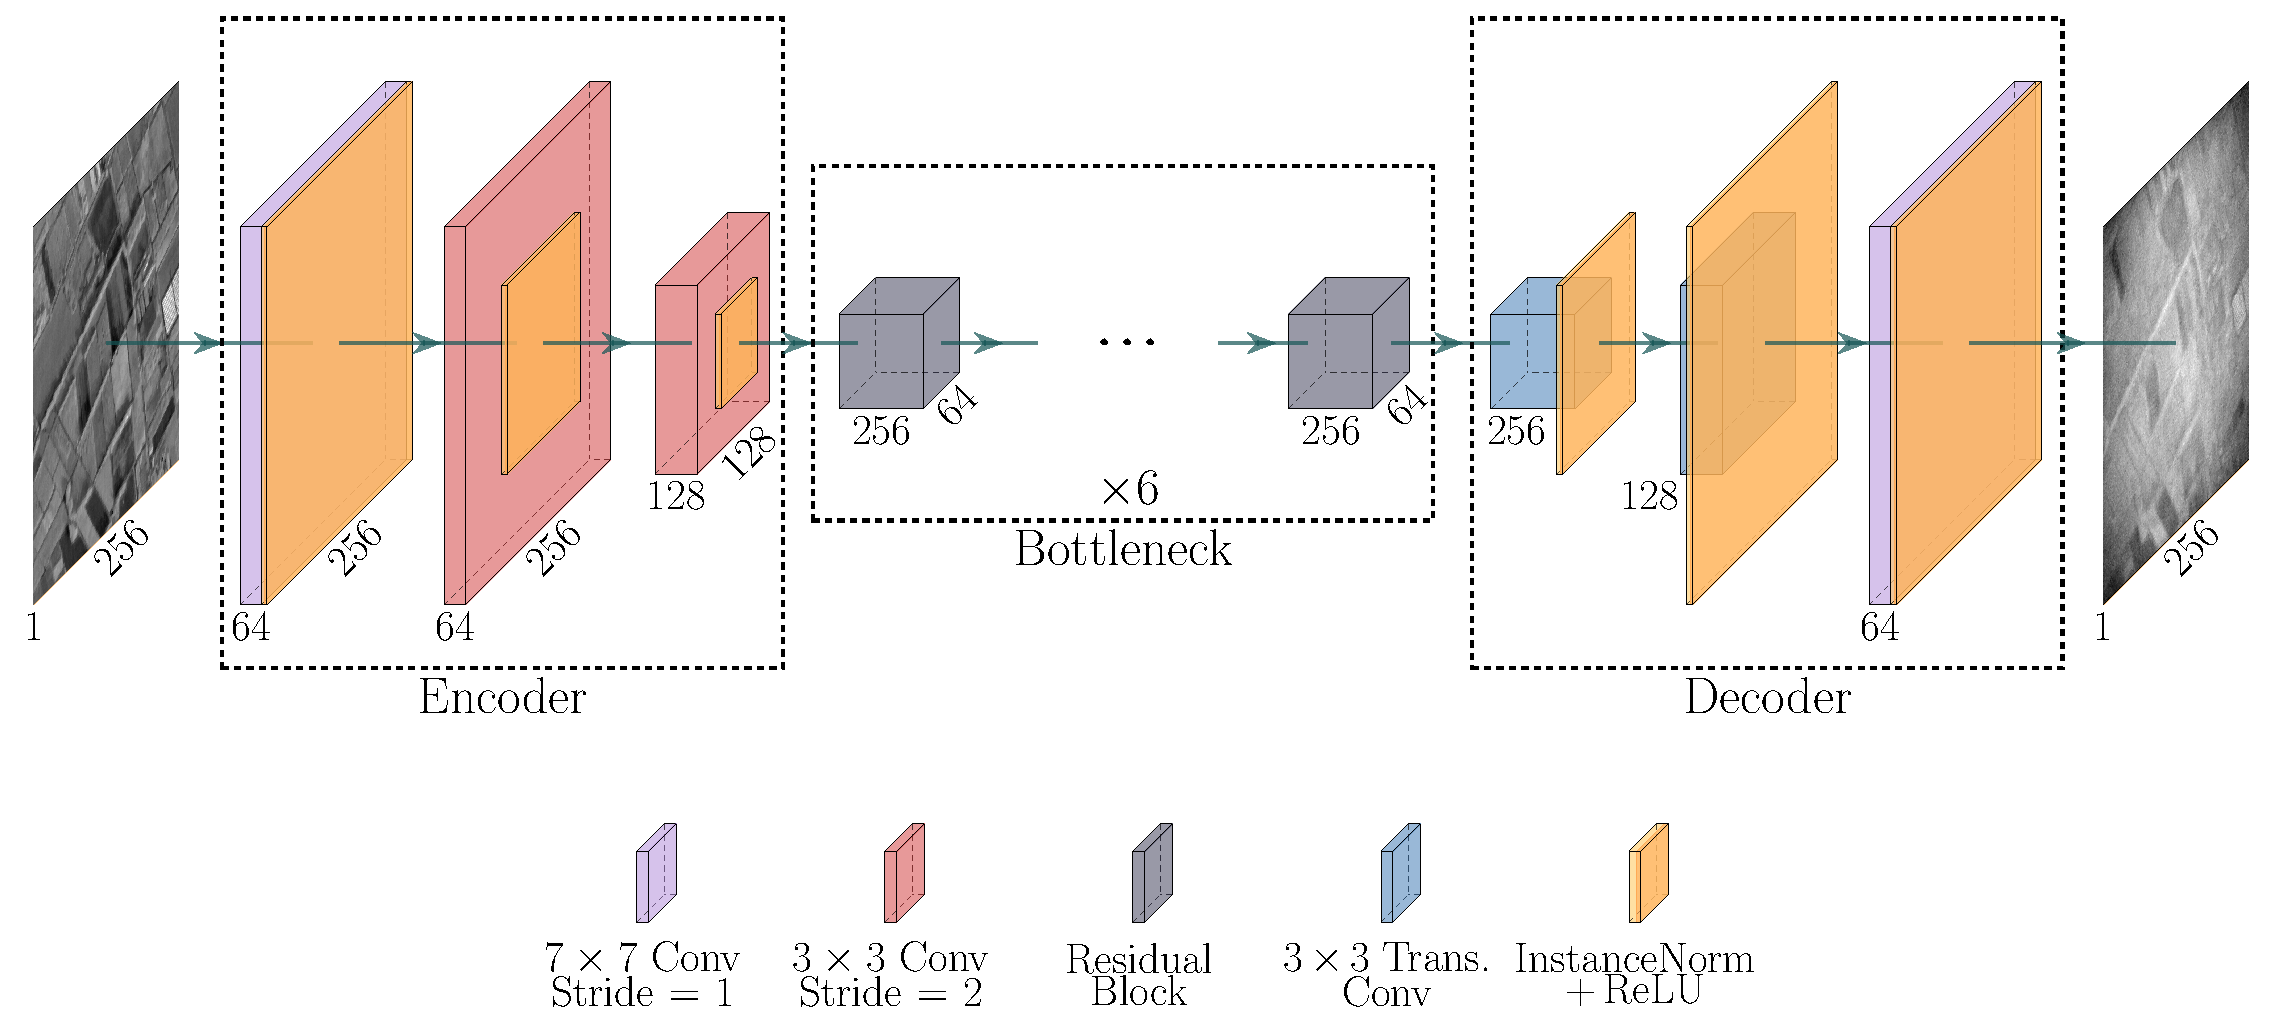
\includegraphics[width=\linewidth]{../figs/network/src/cut.pdf}
    \subcaption{Baseline}
    \label{fig:backbone_models}
    \vspace{0.0cm}
  \end{subfigure}  
  \begin{subfigure}{\textwidth}
    \centering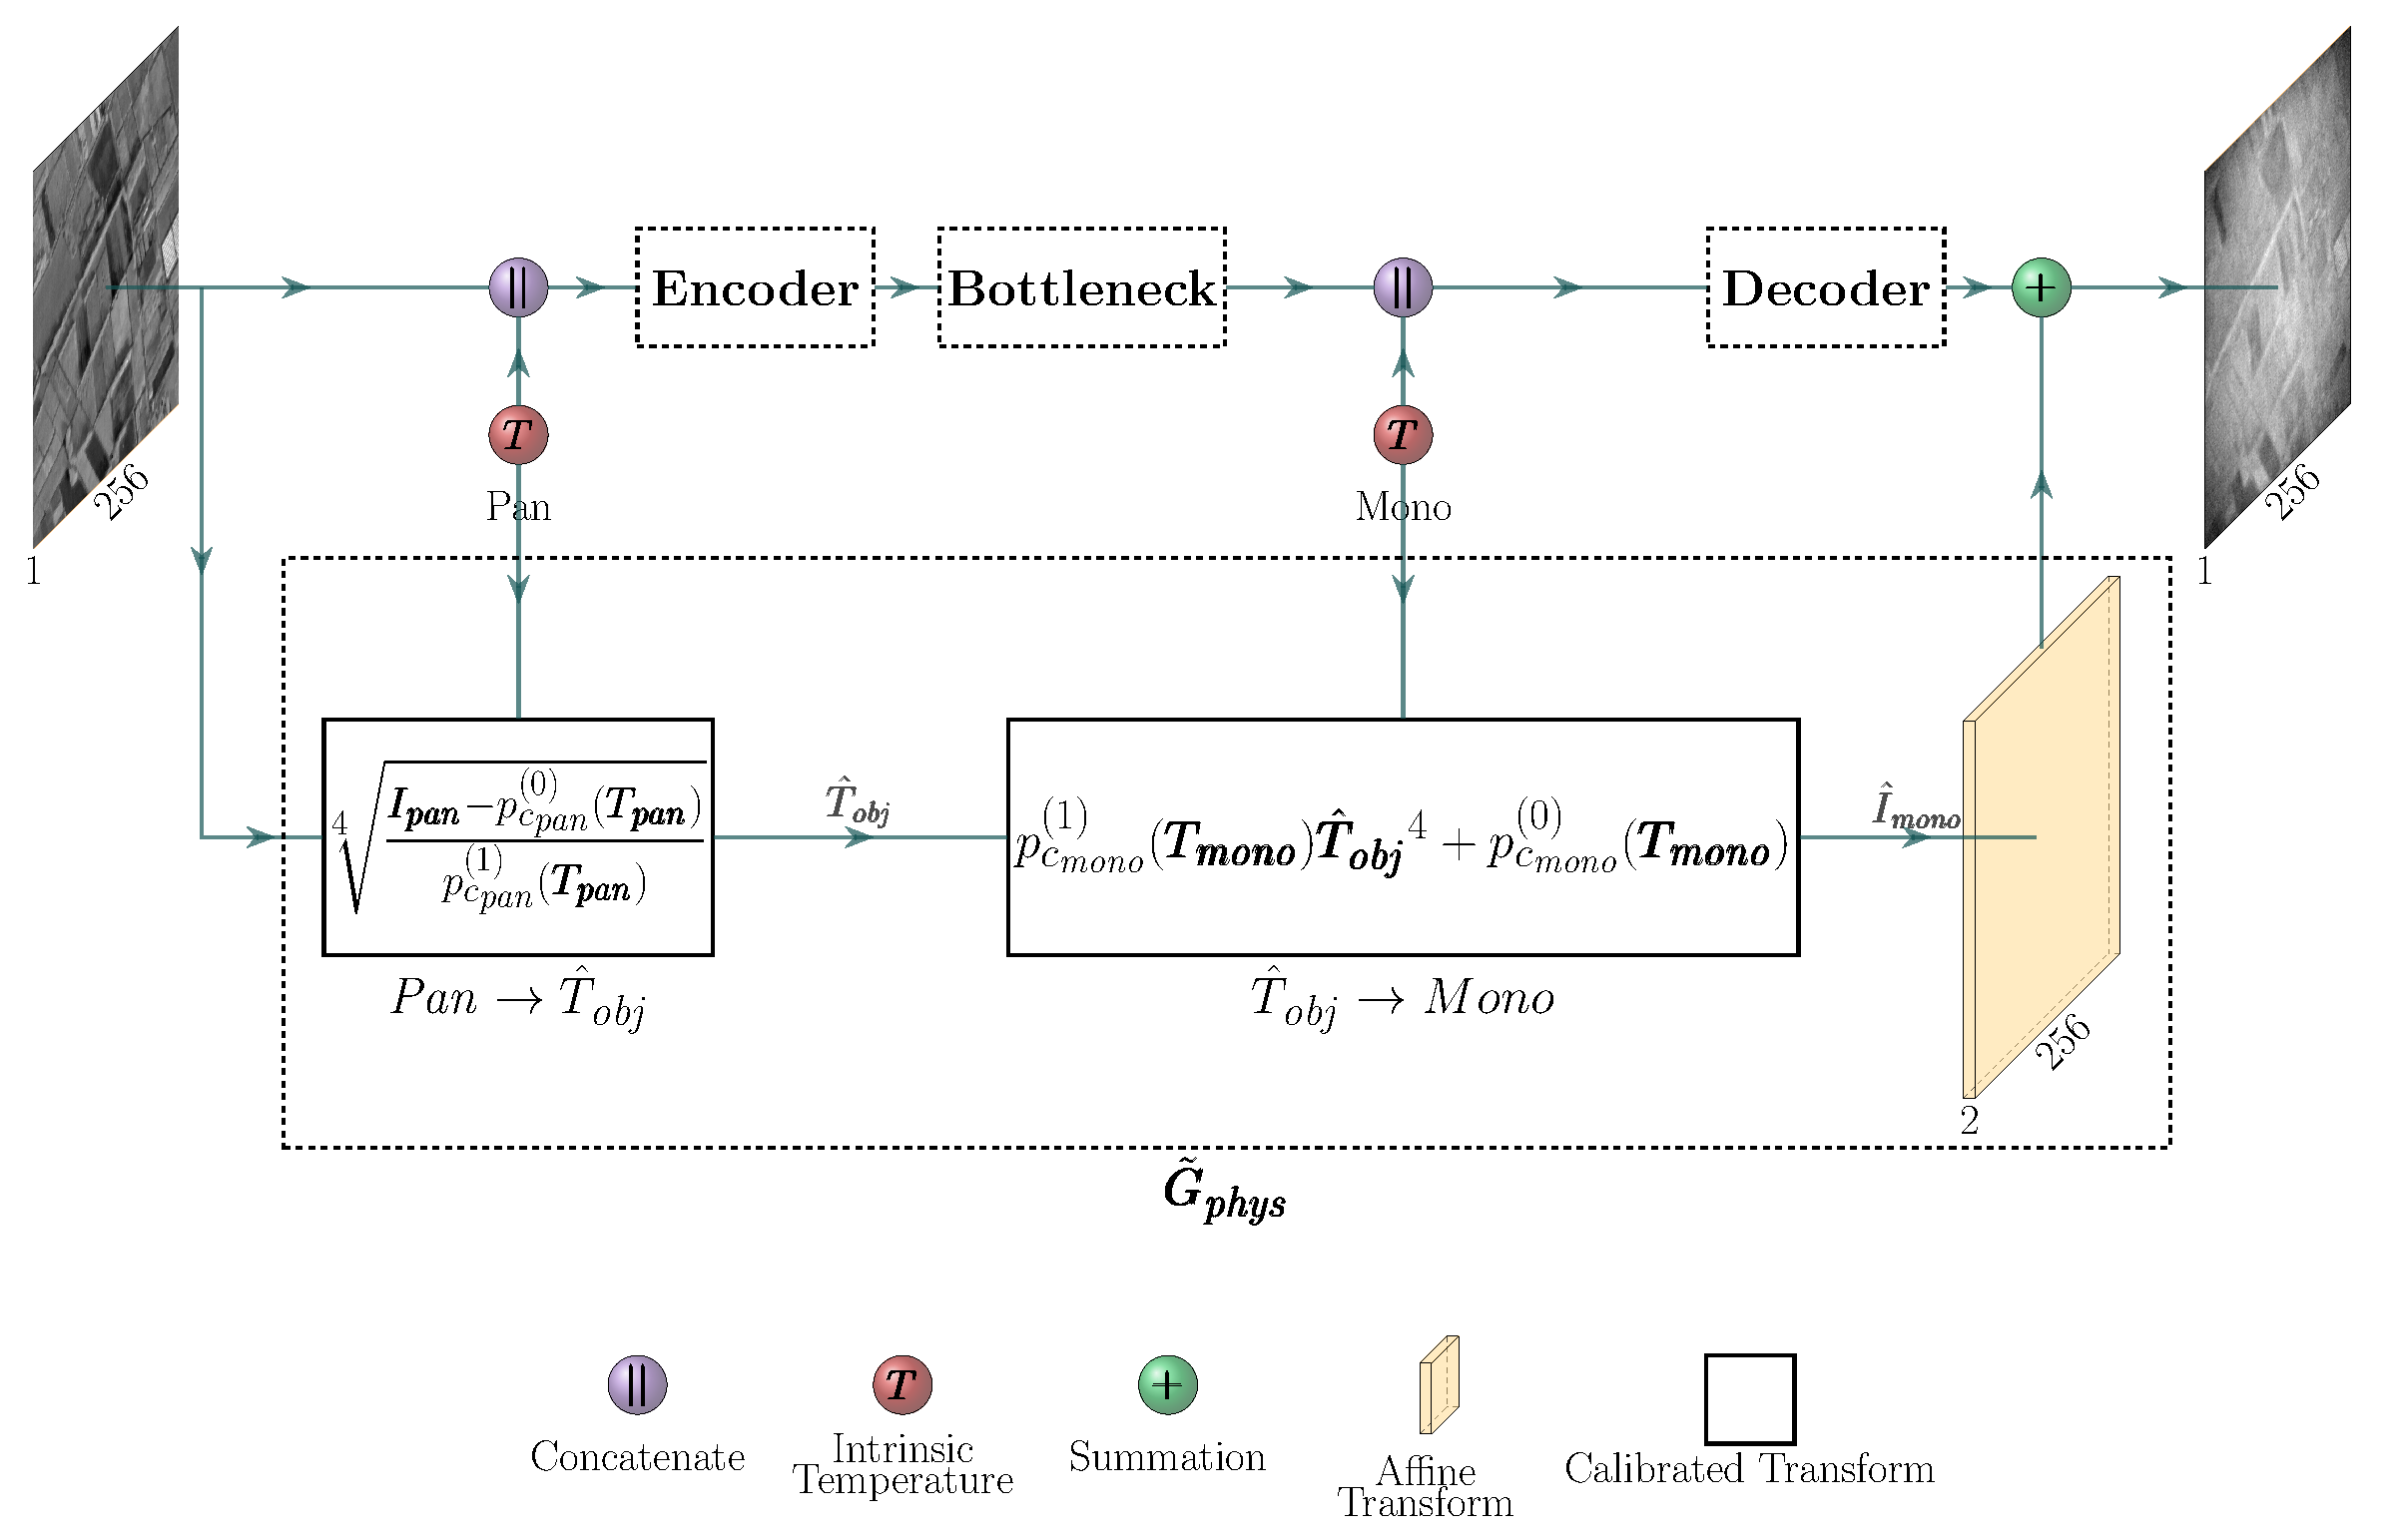
\includegraphics[width=\linewidth]{../figs/network/src/petit.pdf}
    \subcaption{PETIT}
    \label{fig:PETIT_model}
  \end{subfigure}
  \caption{Comparison between the baseline (CycleGAN, CUT) and PETIT (our method) generators. The architectures of the encoder, bottleneck and decoder blocks are identical in all models.}
  \label{fig:arch_comp}
\end{figure}